\cleardoublepage

\chapter{Aplicación desarrollada}
\label{makereference5}

En este capítulo se introducirá la aplicación que se ha desarrollado con el
fin de demostrar los conceptos expuestos en los capítulos anteriores. En
concreto se desarrollarán shaders para los siguientes problemas:

\begin{itemize}
		\item Coloreado de terrenos
		\item Curvas de Bézier
		\item Superficies de Bézier
		\item Sólidos de revolución
		\item Nubes de puntos
		\item Negativo de una imagen
		\item Detección de bordes en una imagen
		\item Line Integral Convolution
\end{itemize}

Para el desarrollo de la aplicación y los shaders será necesario introducir
algunos conceptos matemáticos importantes, que se explican en la
sección~\ref{makereference5.1}.

\section{Plan de desarrollo}
\label{makereference5.1}

Durante las primera semanas de desarrollo de la aplicación lo más importante fue
realizar un exhaustivo estudio del funcionamiento de OpenGL, así como la lectura
y realización de tutoriales sobre la materia. Una vez adquirido el conocimiento
necesario, se comenzó a desarrollar el esqueleto principal de la aplicación,
sobre el cual se incorporarían después los distintos tipos de visualización a
realizar.

Una vez desarrollado este esqueleto se comenzó a la preparación de los shaders
que se utilizarían en cada uno de los problemas, para lo que se utilizó en gran
medida la información expuesta en el texto~\citet{Bailey}.

El siguiente paso fue conseguir datos y prepararlos adecuadamente para poder
mostrar las capacidades de visualización de la aplicación, así como comprobar su
correcto funcionamiento.

Lo anterior fue reiterado con cada uno de los problemas, añadiéndose cada vez
más a lo largo del desarrollo de todo el proyecto.

\section{Herramientas de desarrollo}
\label{makereference5.2}

Como entorno de desarrollo principal se ha utilizado el sistema operativo Ubuntu
Linux 18.04 LTS~\cite{UBUNTU}. En este sistema, además, se han utilizado las
siguientes herramientas de desarrollo:

\begin{itemize}
		\item Vim como editor de textos.~\cite{VIM}
		\item Git para el control de versiones.~\cite{GIT}
		\item Github como respositorio.~\cite{GITHUB}
		\item GCC como compilador.~\cite{GCC}
		\item GDB para la depuración.~\cite{GDB}
		\item Make para la gestión de dependencias.~\cite{MAKE}
\end{itemize}. 

Asimismo, siguiendo las recomendaciones del tutorial~\citet{LearnOpenGL}, se han
utilizado las siguientes librerías:

\begin{itemize}
		\item GLFW~\cite{GLFW}. GLFW es una librería orientada específicamente a
				OpenGL que proporciona las necesidades básicas para el
				renderizado en pantalla. Permite crear un contexto de OpenGL,
				definir parámetros de ventana y manejar la entrada del usuario.
				Estas son las funciones que utilizaremos en la aplicación.
		\item GLAD~\cite{GLAD}. La localización de funciones de OpenGL depende
				tanto del controlador gráfico utilizado como del sistema
				operativo utilizado. Esta localización es desconocida en tiempo
				de  compilación y ha de ser conseguida en tiempo de ejecución.
				Es, pues, tarea del programador conseguir la localización de
				estas funciones. GLAD es una  librería que realiza esta tarea
				automáticamente.
		\item Assimp~\cite{ASSIMP}. Assimp --- \textit{The
				Open-Asset-Importer-Lib} --- es una librería que permite
				importar diferentes formatos de modelos 3D de una manera
				uniforme. Será utilizado para cargar los modelos para el
				colorado de terrenos.
		\item GLM~\cite{GLM}. GLM --- OpenGL Mathematics --- es una librería
				para matemáticas en software gráfico en C++ basada en las
				especificaciones del lenguaje GLSL. Proporciona funciones
				diseñadas e implementadas con el mismo convenio de nombres y
				funcionalidades que GLSL. Proporciona capacidades como
				transformaciones de matrices, cuaterniones, empaquetado de
				datos, aleatoriedad, ruido\ldots
		\item Otras librerías especificas del sistema operativo, como Pthreads,
				xrandr, x11, xi, xcursor, etc.
\end{itemize}

\section{Diseño de la aplicación}
\label{makereference5.3}

Para esta aplicación se ha optado por un diseño modular orientado a objetos, en
el que poder incrementalmente añadir distintos tipos de visualización sin tener
demasiados problemas. Como se ha expuesto en la sección~\ref{makereference5.1}
la aplicación consta de un esqueleto principal utilizado por todos los tipos de
visualización. Este esqueleto consta de una ventana principal, creada en el
programa principal, en la que se renderizará el objeto particular que representa
el tipo de visualización. Así, con el fin de añadir un nuevo tipo de
visualización solo se habrían de realizar las siguientes acciones:

\begin{enumerate}
		\item Crear un nuevo objeto que implemente los métodos necesarios
				de la clase \verb|Object|.
		\item Añadir un nuevo modo al \verb|enum Modes|.
		\item Añadir las opciones necesarias para dicho objeto en el programa
				principal e incluir la nueva clase \verb|#include "class.h"|.
		\item Actualizar las dependencias en el Makefile.
\end{enumerate}

En esta ventana principal se tiene por defecto un sistema de cámara en primera
persona, con la capacidad de moverse para visualizar mejor detalles del objeto
en cuestión. Este sistema puede ser sobreescrito en el objeto específico en
caso de necesitar otro comportamiento. 

En la clase \verb|Object| existen tres métodos virtuales puros, que han de ser
implementados por las clases específicas de cada tipo de visualización:


\begin{itemize}
		\item \verb|draw()|, que ha de encargarse de dibujar el objeto en
				cuestión.
		\item \verb|processInput(GLFWwindow * window)|, que ha de especificar que
				hacer con la entrada del usuario para este tipo de
				visualización.
		\item \verb|setUniforms()|, que ha de especificar las variables
				\verb|uniform| que utilicen los shaders de este tipo de
				visualización.
\end{itemize}

Estos métodos se llaman una vez por vuelta del bucle principal. En la sección
siguiente se introducen las matemáticas necesarias e importantes para el
desarrollo de la aplicación y los shaders concretos.

\section{Matemáticas necesarias}
\label{makereference5.4}

Con el fin de desarrollar el sistema de cámaras que utiliza la aplicación es
necesario conocer varios conceptos importantes sobre álgebra, geometría lineal y
y proyectiva y transformaciones matriciales, así como los ángulos de Euler y su
relación con los cuaterniones. También se explorarán distintos métodos
numéricos, relevantes en el método de Line Integral Convolution, así como
fórmulas matemáticas específicas de cada tipo de visualización.

\subsection{Transformaciones matriciales}
\label{makereference5.4.1}

Como vamos a trabajar con objetos tridimensionales y una cámara móvil,
necesitamos realizar transformaciones sobre los vértices que componen nuestros
objetos para que estos aparezcan en su lugar y con sus dimensiones adecuadas.
Es deseable, además, realizar estas operaciones con vectores matricialmente,
puesto que éstas permiten presentar transformaciones arbitrarias en un
formato consistente y apto para la computación. Así, se pueden concatenar
diferentes transformaciones de manera sencilla multiplicando sus matrices. 

Entre estas transformaciones podemos encontrar lineales y no lineales. Sin
embargo, las transformaciones no lineales y proyectivas no se pueden representar
con una matriz de dimensión la dimensión del espacio Euclídeo. Así, para
representar matricialmente transformaciones no lineales en un espacio Euclídeo
$n$-dimensional $\mathbb{R}^n$ se ha de utilizar una transformación lineal en el
espacio $(n+1)$-dimensional $\mathbb{R}^{n+1}$. Esta es la razón por la que
utilizaremos geometría proyectiva y \textit{coordenadas homogéneas} en la
aplicación.

En esta sección se presentan las coordenadas homogéneas y transformaciones
lineales y afines más habituales y necesarias para nuestra aplicación, así como
sus formas matriciales. 

\subsubsection{Coordenadas Homogéneas}
\label{ref:HomogeneousCoordinates}

Las coordenadas homogéneas son un sistema de coordenadas utilizado en geometría
proyectiva, del mismo modo que las coordenadas cartesianas se utilizan en la
geometría Euclídea. Tienen la ventaja de que las coordenadas de todos los puntos
del espacio, incluidos los puntos en el infinito, se pueden representar mediante
coordenadas finitas.

Debido a que este sistema permite la representación de puntos en el infinito, el
número de coordenadas necesarias para permitirlo ha de ser uno más que la
dimensión del espacio proyectivo considerado. Este sistema, además, permite la
representación de transformaciones afines y proyectivas de forma matricial,
proporcionando un método rápido y eficiente de calcular proyecciones
consecutivas. Como en nuestra aplicación estamos interesados principalmente en
el espacio tridimensional, las matrices que utilizaremos serán $4 \times 4$. Y
los puntos se representarán con $4$ coordenadas. Cabe destacar algunas de las
propiedades de las coordenadas homogéneas antes de continuar con las
transformaciones que vamos a utilizar.

\begin{itemize}

		\item Un punto en el espacio tridimensional está representado por $4$
				coordenadas homogéneas $(x,y,z,w)$, donde $x,y,z$ y $w$ no son
				todas $0$.

		\item Dos conjuntos de coordenadas homogéneas $p$ y $q$ que cumplen la
				relación $p = a \dot q, a \in \mathbb{R}$, es decir, que sólo se
				diferencian en la multiplicación por un escalar, representan el
				mismo punto en el espacio.

		\item Si $w \neq 0$, entonces el punto representado es el punto
				$(\frac{x}{w},\frac{y}{w},\frac{z}{w})$ del espacio Euclídeo
				tridimensional.

		\item Si $w = 0$, entonces el punto representado en un punto del
				infinito.

\end{itemize}

\subsubsection{Traslación}
\label{makereference5.4.1.1}

Se denomina traslación a la operación consistente en \textit{mover} un vector en
una posición a otra nueva posición. Supongamos, pues, que queremos trasladar un
vector $\overrightarrow{v} = (x,y,z)$ en la dirección marcada por el vector
$\overrightarrow{t} = (t_1, t_2, t_3)$ como se muestra en la
figura~\ref{fig:traslation}. Para ello realizaríamos la siguiente operación:

\begin{figure}
	\centering	
	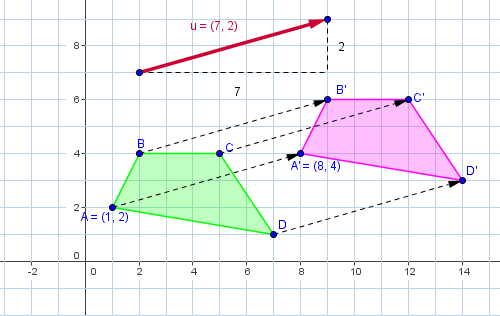
\includegraphics[height=9cm]{figures/traslacion.png}
	\caption[Traslación de un vector.]{Traslación de un vector.
	Fuente:~\cite{vectortraslationimage}}
	\label{fig:traslation}
\end{figure}

\begin{equation}
	\label{eq:translation}
	\overrightarrow{v}' = \overrightarrow{v} + \overrightarrow{t} = 
	\left( \begin{array}{c}
			x + t_1 \\
			y + t_2 \\
			z + t_3 \\
	\end{array} \right)
\end{equation}

La traslación se trata de una transformación afín sin puntos fijos. Como se ha
expuesto previamente, para poder representar esta transformación de forma
matricial se ha de recurrir a un espacio de una dimensión más. Por tanto, se
recurre a las coordenadas homogéneas para representar la traslación de un
espacio vectorial con multiplicación de matrices. Escribiendo el vector
$\overrightarrow{v} = (x,y,z)$ utilizando una cuarta coordenada homogénea
$\overrightarrow{v} = (x,y,z,1)$. Esta operación se muestra
en~\eqref{eq:matrixtranslation}. 

\begin{equation}
	\label{eq:matrixtranslation}
	\overrightarrow{v}' = 
	\left( \begin{array}{cccc}
			1 & 0 & 0 & t_1 \\
			0 & 1 & 0 & t_2 \\
			0 & 0 & 1 & t_3 \\
			0 & 0 & 0 & 1 \\
	\end{array} \right)
	\left( \begin{array}{c}
			x \\
			y \\
			z \\
			1 \\
	\end{array} \right) = 
	\left( \begin{array}{c}
			x + t_1 \\
			y + t_2 \\
			z + t_3 \\
			1 \\
	\end{array} \right)
\end{equation}\\

\subsubsection{Escalado}
\label{makereference5.4.1.2}

El escalado de un vector es la operación consistente en modificar la longitud
del vector. Para ello, debemos multiplicar cada una de sus coordenadas por el
factor de escalado deseado en cada eje. Es decir, para escalar un vector
$\overrightarrow{v}$ por un factor de $0.5$ en el eje $x$ y $3$ en el eje $y$,
la operación a realizar sería la siguiente:

\begin{equation}
	\label{eq:scaling}
	\overrightarrow{v} = 
	\left( \begin{array}{c}
			2 \\
			3 \\
	\end{array} \right)
	\;\;\;\;\;
	\overrightarrow{v}' =
	\left( \begin{array}{c}
		2\cdot0.5 \\
		3\cdot3 \\
	\end{array}	\right) =  
	\left( \begin{array}{c}
			1 \\
			9 \\
	\end{array} \right)
\end{equation}\\

\begin{figure}[ht]
	\centering
	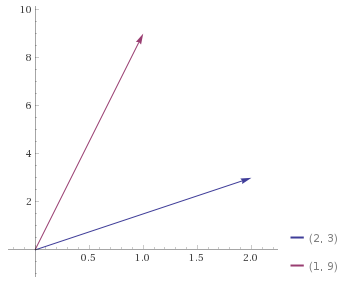
\includegraphics{figures/scaling.png}
	\caption[Escalar un vector.]{Escalar un vector. Fuente:~\cite{wolfram}}
	\label{fig:scaling}
\end{figure}

Esta operación de escalado se puede escribir matricialmente en coordenadas
homogéneas como sigue.  Supongamos que tenemos un vector
$\overrightarrow{v}=(x,y,z)$ y lo queremos escalar por un factor
$fac=(F_1,F_2,F_3)$. Entonces podemos escribir la operación anterior con la
matriz $FAC$ como sigue:

\begin{equation}
	\label{eq:matrixscaling}
	\overrightarrow{v}' = 
	\left( \begin{array}{cccc}
			F_1 & 0   & 0   & 0	\\
			0   & F_2 & 0   & 0	\\
			0   & 0   & F_3 & 0	\\
			0   & 0   & 0   & 1	\\
	\end{array} \right)
	\left( \begin{array}{c}
			x \\
			y \\
			z \\
			1 \\
	\end{array} \right) =
	\left( \begin{array}{c}
			F_1\cdot x \\
			F_2\cdot y \\
			F_3\cdot z \\
			1 \\
	\end{array} \right)
\end{equation}\\

\subsubsection{Rotación}
\label{makereference5.4.1.3}

Al contrario de los casos de la rotación y traslación de vectores expuestas
anteriormente, el caso de la rotación requiere un estudio más profundo en el
caso tridimensional para la matemática aplicada. Por esto, se dedica una sección
exclusiva para este tema. (Ver sección~\ref{makereference5.4.2}).

\subsubsection{Perspectiva}
\label{ref:ProjectionMatrix}

Además de las transformaciones anteriores, se hace necesario realizar una
última, muy importante en el caso de la visualización. Se trata de la
perspectiva. Con esta transformación se conseguirá que los objetos más lejanos
aparezcan más pequeños mientras que los más cercanos aparecerán más grandes.

En la creación de esta matriz aparecen diferentes parámetros a tener en cuenta,
que son los siguientes:

\begin{itemize}
		\item $aspect$ - El ratio entre la anchura y altura del rectángulo en el que se
				realizará esta proyección
		\item $fov$ - El campo de visión vertical. Es el ángulo vertical de la cámara
				mediante la que estamos viendo la escena
		\item $near$ - La localización del plano Z cercano. Se utiliza para realizar
				clipping sobre los objetos que quedan demasiado cerca de la
				cámara
		\item $far$ - La localización del plano Z lejano. Se utiliza para realizar
				clipping sobre los objetos que quedan demasiado lejos de la
				cámara
\end{itemize}

La matriz correspondiente a esta transformación es la siguiente:

\begin{equation}
	\left( 
		\begin{array}{cccc}
				\frac{1}{aspect*\tan{\frac{fov}{2}}} & 0 & 0 & 0 \\
				0 & \frac{1}{\tan{\frac{fov}{2}}} & 0 & 0 \\
				0 & 0 & -\frac{far+near}{far-near} & - \frac{2far \cdot near}{far
				- near} \\
				0 & 0 & -1 & 0 \\
		\end{array}	
	\right)
\end{equation}

La derivación de esta matriz puede verse en~\citet{projectionmatrix}.

\begin{figure}[ht]
	\centering	
	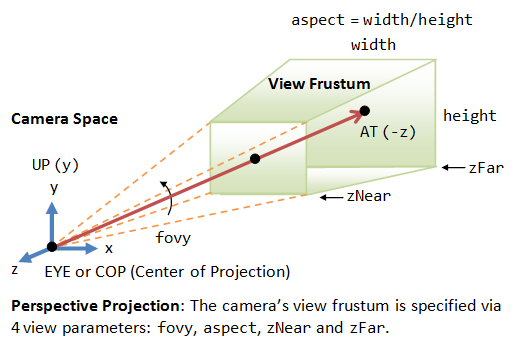
\includegraphics[height=8cm]{figures/projectionimage.png}
	\caption[Proyección perspectiva - Parámetros y significado.]{Proyección
	perspectiva - Parámetros y significado. Fuente:~\cite{projectionimage}}
	\label{fig:projectionimage}
\end{figure}

\subsection{Rotación: Ángulos de Euler y Cuaterniones}
\label{makereference5.4.2}

La rotación tridimensional es un caso particularmente complejo. Esto se debe a
determinados problemas que surgen a la hora de formalizar matemáticamente este
movimiento. 

La manera más intuitiva de pensar en la rotación consiste en especificar esta
rotación mediante un eje de giro y un ángulo. Con esto, el movimiento
consistiría en rotar el vector en torno al eje de giro. (Ver
Figura~\ref{fig:rotacion}). 

Existen diversas maneras de formular matemáticamente este movimiento. Para ello
existe un grupo, llamado $SO(3)$, que es el grupo de todas las rotaciones en
torno al origen del espacio vectorial Euclídeo $\mathbb{R}^3$ bajo la operación
de la composición. Una rotación en $\mathbb{R}^3$ es una aplicación lineal. Como
toda aplicación lineal en un espacio vectorial, ésta puede ser representada
mediante una matriz, dando lugar a la representación matricial de la rotación.

\begin{figure}
	\centering		
	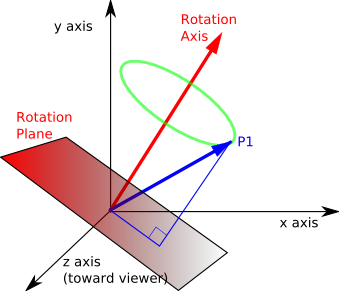
\includegraphics[height=9.5cm]{figures/rotation.png}
	\caption[Rotación de un vector 3D.]{Rotación de un vector 3D.
	Fuente:~\cite{rotationimage}}
	\label{fig:rotacion}
\end{figure}

\subsubsection{Ángulos de Euler y Matriz de rotación}
\label{makereference5.4.2.1}

En el espacio vectorial $\mathbb{R}^3$, los vectores se representan a partir de
una base. Esta base estará formada por tres vectores unitarios. Por tanto, si
queremos realizar una rotación de cualquier otro vector en $\mathbb{R}^3$,
bastará con rotar los vectores de la base acorde al eje de rotación y después
calcular el vector a rotar en términos de la base rotada. 

Los vectores rotados que forman la nueva base definen completamente la rotación
y, escritos como una matriz nos da la matriz de rotación. Esta matriz, al ser
los vectores una base ortonormal de $\mathbb{R}^3$, forman una matriz ortogonal.
Por tanto, el grupo $SO(3)$ se identifica con el grupo formado por las matrices
ortogonales $3\times 3$ bajo la operación de la multiplicación. Estas matrices
se conocen como \textit{Matrices Ortogonales Especiales (Special Orthogonal
Matrices)}, de ahí la notación de $SO(3)$. 

Como sabemos, dos rotaciones en $SO(3)$ se pueden concatenar mediante la
composición, dando lugar a otra nueva rotación. Lo mismo pasa con la
representación matricial, multiplicando dos matrices de rotación. Para nuestra
aplicación, es conveniente realizar las rotaciones como composición de
rotaciones en torno a los ejes de referencia. Para ello definimos las matrices
de rotación, de nuevo utilizando coordenadas homogéneas acorde a lo explicado
anteriormente. 

\begin{equation}
	R_x(\theta) =
	\left(	
		\begin{array}{cccc}
			1 & 0 & 0 & 0 \\				
			0 & \cos{\theta} & -\sin{\theta} & 0 \\				
			0 & \sin{\theta} & \cos{\theta} & 0 \\				
			0 & 0 & 0 & 1 \\				
		\end{array}
	\right)
\end{equation}

\begin{equation}
	R_y(\theta) =
	\left(	
		\begin{array}{cccc}
			\cos{\theta} & 0 & \sin{\theta} & 0 \\				
			0 & 1 & 0 & 0 \\				
			-\sin{\theta} & 0 & \cos{\theta} & 0 \\				
			0 & 0 & 0 & 1 \\				
		\end{array}
	\right)
\end{equation}

\begin{equation}
	R_z(\theta) =
	\left(	
		\begin{array}{cccc}
			\cos{\theta} & -\sin{\theta} & 0 & 0 \\				
			\sin{\theta} & \cos{\theta} & 0 & 0 \\				
			0 & 0 & 1 & 0\\				
			0 & 0 & 0 & 1 \\				
		\end{array}
	\right)
\end{equation} 

Esto da lugar a los conocidos como ángulos de Euler, llamados en inglés
\textit{yaw, pitch, roll}. (Ver Figura~\ref{fig:eulerangles}). Así, una rotación
cualquiera en el espacio tridimensional viene dada por:

\begin{figure}
	\centering
	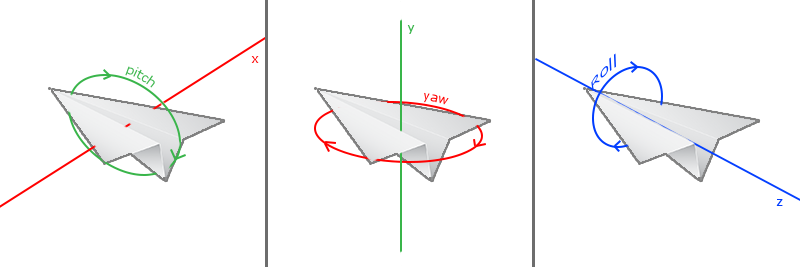
\includegraphics[height=7.5cm,width=\textwidth]{figures/eulerangles.png}
	\caption[Ángulos de Euler.]{Ángulos de Euler. Fuente:~\citet{LearnOpenGL}}
	\label{fig:eulerangles}
\end{figure}

\begin{equation}
		R = Roll(\phi)Pitch(\theta)Yaw(\varphi) = R_x(\phi)R_y(\theta)R_z(\varphi)	
\end{equation}

Ahora bien, existen diversos problemas derivados de la utilización de este
sistema. El más importante es el llamado Bloqueo del
Cardán~\cite{Vince:2011:QCG:2016678}. Aunque los formalismos matemáticos son más
complejos, intuitivamente este bloqueo ocurre debido a que la descripción de
cualquier rotación tridimensional mediante ángulos de Euler no es única y
existen puntos sobre los que no todo cambio en el espacio de rotaciones puede
ser expresado mediante cambios en el espacio de los ángulos de Euler. 

Con el fin de disminuir el riesgo del bloqueo, se puede prescindir de la
multiplicación de matrices utilizando una sola matriz utilizando un eje de giro
arbitrario unitario $u = (u_x, u_y, u_z)$ y un ángulo de giro $\theta$. La
procedencia de dicha matriz se puede consultar en~\citet{Rodrigues}. 

\begin{equation}
		R = 
		\left(
				\begin{array}{cccc}
						\cos\theta + u_x^2(1-\cos\theta) &
						u_xu_y(1-\cos\theta)-u_z\sin\theta &
						u_xu_z(1-\cos\theta)+u_y\sin\theta & 0 \\

						u_yu_x(1-\cos\theta)+u_z\sin\theta & \cos\theta +
						u_y^2(1-\cos\theta) &
						u_yu_z(1-\cos\theta)-u_x\sin\theta & 0 \\

						u_zu_x(1-\cos\theta)-u_y\sin\theta &
						u_zu_y(1-\cos\theta) + u_x\sin\theta & \cos\theta +
						u_z^2(1-\cos\theta) & 0 \\

						0 & 0 & 0 & 1 \\
				\end{array}
		\right)
\end{equation}

\subsubsection{Cuaterniones}
\label{makereference5.4.2.2}

Debido a la importancia de la precisión en muchos sistemas informáticos que
necesitan cálculos de rotaciones y el problema que supone el bloqueo del Cardán,
se hace importante la mención de los cuaterniones como sistema de representación
de rotaciones en tres dimensiones, aunque no los vayamos a utilizar en nuestra
aplicación. 

Los cuaterniones, también conocidos como cuaternios, suponen una notación para
representar orientaciones y rotaciones en tres dimensiones. En contraposición
con los ángulos de Euler, son más sencillos de componer y previenen el bloqueo
del Cardán. Comparados con las matrices de rotación, suponen un método más
compacto, más estable numéricamente y más eficiente. 

Los cuaterniones son una extensión de los números complejos, descritos por
primera vez por William Rowan Hamilton en 1843, definiéndolos como el cociente
de dos lineas dirigidas en un espacio tridimensional.  Cuando se utilizan para
representar rotaciones se les denomina también cuaterniones de rotación, puesto
que representan el grupo $SO(3)$. 

Generalmente, se representan de la siguiente forma:

\[a + b\boldsymbol{i} + c\boldsymbol{j} + d\boldsymbol{k} \] 

donde $a,b,c$ y $d$ son números reales y $\boldsymbol{i}, \boldsymbol{j}$ y
$\boldsymbol{k}$ son las unidades fundamentales del cuaternión. Además, los
cuaterniones  siguen las reglas algebraicas usuales, excepto la de la propiedad
conmutativa de la multiplicación, y cumplen la siguiente propiedad:

\[\boldsymbol{i}^2 = \boldsymbol{j}^2 = \boldsymbol{k}^2 = \boldsymbol{ijk} = -1 \]

Es conveniente verlos representados como un escalar más un vector, es decir:

\[a + b\boldsymbol{i} + c\boldsymbol{j} + d\boldsymbol{k} = a +
\overrightarrow{v} \] 

considerando la parte imaginaria $b\boldsymbol{i} + c\boldsymbol{j} +
d\boldsymbol{k}$ como un vector $\overrightarrow{v} = (b,c,d)$. 

Recordemos que cualquier rotación en el espacio tridimensional puede verse como
una giro de ángulo $\theta$ en torno a un eje definido por un vector unitario
$u$. Esto puede ser representado mediante un cuaternión de la siguiente forma:

\[\boldsymbol{q} = \exp{\frac{\theta}{2}(u_x\boldsymbol{i} + u_y\boldsymbol{j} +
		u_z\boldsymbol{k})} = \cos{\frac{\theta}{2}} + (u_x\boldsymbol{i} + 
u_y\boldsymbol{j} + u_z\boldsymbol{k})\sin{\frac{\theta}{2}} \]

Se puede demostrar que un la rotación deseada se puede aplicar a un vector
ordinario $\boldsymbol{p} = (p_x, p_y, p_z) = p_x\boldsymbol{i} +
p_y\boldsymbol{j} + p_z\boldsymbol{k}$ en el espacio tridimensional, considerado
como un cuaternión con parte real igual a cero, evaluando la conjunción de
$\boldsymbol{p}$ por $\boldsymbol{q}$:

\[ \boldsymbol{p'} = \boldsymbol{qpq^{-1}} \]

donde $\boldsymbol{p'}$ es la nueva posición del vector $\boldsymbol{p}$ tras la
rotación. La parte vectorial del este cuaternión es el vector deseado. Se puede
leer más acerca de cuaterniones utilizados para las rotaciones en~\citet{Vicci}.

\subsection{Métodos Numéricos para la resolución de Ecuaciones Diferenciales} 
\label{makereference5.4.3}

Como ya se vio en la sección~\ref{ref:lic}, en el método del Line Integral
Convolution se ha de utilizar un método numérico para computar la línea de
flujo. En esta sección se analizan algunos de los métodos utilizados y
propuestos tanto por~\citet{osti_10185520} como por \citet{licthesis}.

Para poder analizar los métodos hemos de introducir algunas definiciones
relacionadas con ellos. Recordemos que un método numérico sirve para calcular de
manera aproximada la solución de una ecuación diferencial en un intervalo $[t_0,
T]$. Para ello, dividiremos el intervalo en una serie de puntos, dando lugar a
los siguientes conceptos~\cite{ANNU}:

\begin{itemize}

		\item \textbf{Puntos de red.} Cada uno de los puntos en los que se
				divide el intervalo $[t_0, T]$. Los subintervalos resultantes
				pueden ser de longitud constante (Redes uniformes de paso
				$h=\frac{T-t_0}{N}$) o de longitud variable, dando lugar a
				los métodos númericos de paso variable.

		\item \textbf{Esquema Numérico.} Se denomina esquema numérico al proceso
				iterativo mediante el cual, conociendo los $r$ primeros valores
				$x_0, x_1, \ldots, x_{r-1}$, que son aproximaciones de los
				valores exactos $x(t_0),x(t_1),\ldots,x(t_{n-1})$ de la solución
				de la ecuación diferencial en los puntos $t_0, t_1, \ldots,
				t_{r-1}$ podemos calcular todos los demás valores $x_n, n =
				r,\ldots,N$, que son aproximaciones de los valores exactos en
				los puntos de red.

				El esquema numérico se escribe de la siguiente forma:

				\begin{equation}
					\left\{ \begin{aligned}
							& x_0,x_1,\ldots,x_{r-1} \; \textrm{dados} \\
							& x_{n-r} = \Phi
							(t_n,x_n,x_{n+1},\ldots,x_{n+r-1},h), \; n =
							0,\ldots,N-r \\
					\end{aligned} \right.
				\end{equation}

		\item \textbf{Error Local de Truncamiento.} Dado un esquema como el
				anterior, suponiendo que las soluciones exactas verifican

				\begin{equation}
						x(t_{n+r}) = \Phi (t_n,
						t_{n+1},\ldots,t_{n+r-1},x(t_n),x(t_{n+1}),\ldots,x(t_{n+r-1}))
						+ h\tau_{n+r}(h)
				\end{equation}

				el error local de truncamiento viene dado por

				\begin{equation}
						\tau (h) := \max_{n=0,\ldots,N-r}|\tau_{n+r}(h)|	
				\end{equation}

				que consiste en el error que se comete al calcular el valor
				exacto utilizando el esquema numérico.

		\item \textbf{Consistencia.} Se dice que un método es consistente si

				\begin{equation}
						\lim_{h\to 0} \tau(h) = 0	
				\end{equation}

				Se dice que es consistente de orden $p$ si

				\begin{equation}
					\tau(h) = O(h^p)				
				\end{equation}

		\item \textbf{Error Global de Discretización.} Siguiendo la notación
				anterior, el Error global de discretización viene dado por

				\begin{equation}
					\epsilon (h) := \max_{n=0,\ldots,N}|x_n - x(t_n)|
				\end{equation}

		\item \textbf{Convergencia.} Se dice que un método es convergente cuando
				se verifica lo siguiente:

				\begin{equation}
						si \;\;\; \max_{k=0,\ldots,r-1}|x_k - x(t_k)|
						\xrightarrow {h\to 0} 0	\;\;\; entonces \;\;\; \lim_{h\to
						0}\epsilon(h) = 0
				\end{equation}

				Se dice que es convergente de orden $p$ si

				\begin{equation}
						\epsilon(h) = O(h^p)	
				\end{equation}

\end{itemize}

Con estas nociones ya podemos empezar a analizar los distintos métodos
utilizados, para así conocer cuáles proporcionarán mejores resultados. 

\subsubsection{Método de Euler}
\label{makereference5.4.3.1}

El método de Euler es el más sencillo de los métodos numéricos a considerar. Se
trata de un método por aproximación de la derivada. Para ver cómo aparece este
método, hemos de recurrir a la definición de derivada. Para cada $t \in (t_0,T)$

\begin{equation}
		x'(t) = \lim_{h \to 0} \frac{x(t+h) - x(t)}{h} 	
\end{equation}

Si $h>0$ es suficientemente pequeño, podemos suponer que

\begin{equation}
		x'(t_n)\approx \frac{x(t_n+h) - x(t_n)}{h} = \frac{x(t_{n+1}) -
		x(t_n)}{h}	
\end{equation}

lo que nos conduce a que

\begin{equation}
		x(t_{n+1}) \approx x(t_n) + hf(t_n,x(t_n))	
\end{equation}

De aquí aparece el esquema numérico del método de Euler

\begin{equation}
		\left\{ \begin{aligned}
				& x_{n+1} = x_n + hf(t_n,x_n) \; n=0,\ldots,N-1 \\
				& x_0 \approx a \\
		\end{aligned} \right.
\end{equation}

En~\citet{ANNU} se puede ver una demostración de que el método de Euler supone
un método \textbf{consistente de orden 1} y \textbf{convergente}.

\subsubsection{Método de Euler de paso variable}
\label{makereference5.4.3.2}

El método de Euler de paso variable sigue la misma idea general que el método de
Euler de paso uniforme. En este caso, sin embargo, el siguiente punto en el que
calcular la solución aproximada se calcula en cada paso. Para ello, se ha de
fijar previamente una tolerancia permitida para el error cometido. Por tanto,
necesitamos ser capaces de \textbf{estimar} el error que vamos a cometer al
escoger el siguiente paso. Entonces, si el error estimado es mayor que la
tolerancia fijada, el cálculo se descarta y se vuelve a realiza, y si éste es
menor que la tolerancia, entonces se acepta y se pasa al siguiente cálculo.

Con el fin de realizar esta estimación, como hemos dicho, necesitamos introducir
los siguientes conceptos:

\begin{itemize}

		\item \textbf{Error local relativo al paso $h$.} Se define el error local relativo
				al paso $h$ en el nodo $t_{n+1} = t_n + h$ como 

				\begin{equation}
						ERR_n(h) := \frac{|y(t_n + h) - y_1(t_n,h)|}{h}	
				\end{equation}

				donde la función $y = y(t)$ es la solución del problema y la
				función $y_1(t_n,h)$ representa la aproximación numérica desde
				el instante $t_n$ en un paso $h$,dada por $y_1(t_n,h) :=  x_n +
				h\Phi (t_n,x_n,h)$ Con esta notación, $x_{n+1} = y_1(t_n,hn+1)$.

		\item \textbf{Error local relativo.} Se define el error local relativo
				como 

				\begin{equation}
						ERR(h_1,\ldots,h_N):=\max_{n=1,\ldots,N-1}|ERR_n(h_n+1)|	
				\end{equation}

\end{itemize}

De nuevo en~\citet{ANNU} podemos encontrar demostrado que si un método de paso
adaptativo es consistente, estable y de orden $p$, entonces

\[\tau(h_1,\ldots,h_N) \le Ch_{max}^p\]

para cierta constante $C$ y, por tanto, si $x_0\to a$ y $h_{max}\to 0$, obtenemos que $\epsilon(h_1,\ldots,h_N)\to 0$.

El esquema para este tipo de métodos es:

\begin{equation}
		\left\{
		\begin{aligned}
			& x_{n+1} = x_n + h_{n+1}\Phi(t_n,x_n,h_{n+1}) \;\;\; n= 0,\ldots,N-1 \\
			& x_0 \sim a \\
		\end{aligned}
		\right.
\end{equation}

El método de Euler adaptativo es, por tanto:

\begin{equation}
		\left\{
		\begin{aligned}
			& x_{n+1} = x_n + h_{n+1}f(t_n,x_n) \;\;\; n= 0,\ldots,N-1 \\
			& x_0 \sim a \\
		\end{aligned}
		\right.
\end{equation}

Este método es propuesto en~\citet{osti_10185520}.

\subsubsection{Métodos de Runge-Kutta}
\label{makereference5.4.3.3}

Los últimos métodos que vamos a considerar, y en particular el que vamos a
implementar en nuestra aplicación para el método del Line Integral Convolution,
son los métodos de Runge-Kutta. Esta familia de métodos se basa en añadir puntos
intermedios entre los puntos del mallado $t_n$ y $t_{n+1}$ en la media
ponderada. 

Como ejemplo, si consideramos una media ponderada entre las pendientes en los
puntos $t_n$ y $t_n + ch$ con $c \in (0,1]$ podemos aproximar el valor de
$x(t_{n+1})$ por 

\[x(t_{n+1}) \approx x(t_n) + h\left[ b_1f(t_n,x(t_n)) + b_2f(t_n + ch,
x(t_n+ch))\right]\]

donde $b_1 + b_2 = 1$, para que sea realmente una media. El problema ahora
radica en cómo calcular el valor $x(t_n +ch)$. Una manera de hacerlo es utilizar
el método de Euler, es decir,

\[x(t_n + ch) \approx x(t_n) + chf(tn,x(t_n))\]

De esta forma, la aproximación de $x(t_{n+1})$ queda:

\[x(t_{n+1}) \approx x(t_n) + h\Big[ b_1f(t_n,x(t_n)) + b_2f\Big(t_n+ch,x(t_n) +
		chf(t_n,x(t_n))\Big)\Big] \]

obteniéndose la familia de métodos Runge-Kutta

\[ x_{n+1} = x_n + h\Big[b_1f(t_n,x_n + b_2f\Big(t_n + ch, x_n +
chf(t_n,x_n)\Big)\Big] \]

que suele escribirse como

\[ \left\{ 
		\begin{aligned}
		& K_1 = f(t_n,x_n) \\
		& K_2 = f(t_n + ch, x_n + chK_1) \\
		& x_{n+1} = x_n + h(b_1K_1 + b_2K_2) \\
		\end{aligned}
	\right. \]

En este caso, el método tiene $2$ etapas. Esta familia de métodos de puede
generalizar, dando lugar a los métodos de Runge-Kutta de $s$ etapas. La
forma de escribir estos métodos es la siguiente:

\begin{equation}
	\left\{	
		\begin{aligned}
			& K_i = f\bigg(t_n + c_ih,x_n + h\sum_{j=1}^sa_{ij}K_j\bigg),
			\;\;\; i=1,2,3,\ldots,s, \\
			& x_{n+1} = x_n + h\sum_{i=1}^sb_iK_i \\
		\end{aligned}
		\right.
\end{equation}

El que vamos a utilizar en nuestra aplicación es el método de Runge-Kutta de
orden 4, que tiene el siguiente esquema numérico:

\begin{equation}
	\left\{	
		\begin{aligned}
			& K_1 = f(t,x) \\
			& K_2 = f\bigg(t+\frac{h}{2},x+\frac{h}{2}K_1\bigg) \\
			& K_3 = f\bigg(t+\frac{h}{2},x+\frac{h}{2}K_2\bigg) \\
			& K_4 = f\Big(t+h,x+hK_3\Big) \\
			& x_{n+1} = x_n + \frac{h}{6}[K_1 + 2K_2 + 2K_3 + K_4] \\
		\end{aligned}
	\right.
\end{equation}

La demostración de que este método es consistente de orden 4 se puede encontrar
en~\citet{ANNU}.

\subsection{Otras Fórmulas}
\label{makereference5.4.4}

Para el desarrollo de la aplicación también se han tenido que utilizar fórmulas
matemáticas que describen el comportamiento de las curvas y superficies de
Bézier, ya explicadas en la sección~\ref{ref:bezier}, así como las
fórmulas para la obtención de los valores de los píxeles de salida en el método
del Line Integral Convolution (Sección~\ref{ref:lic}).

\section{Shaders en la aplicación}
\label{makereference5.5}

En esta sección se presentan ya los shaders desarrollados para cada uno de los
tipos de visualización considerados en el proyecto, analizando los distintos
cálculos realizados y explorando las entradas y salidas de cada uno de ellos.

\subsection{Coloreado de terrenos}
\label{makereference5.5.1}

\begin{figure}[ht]
	\centering
	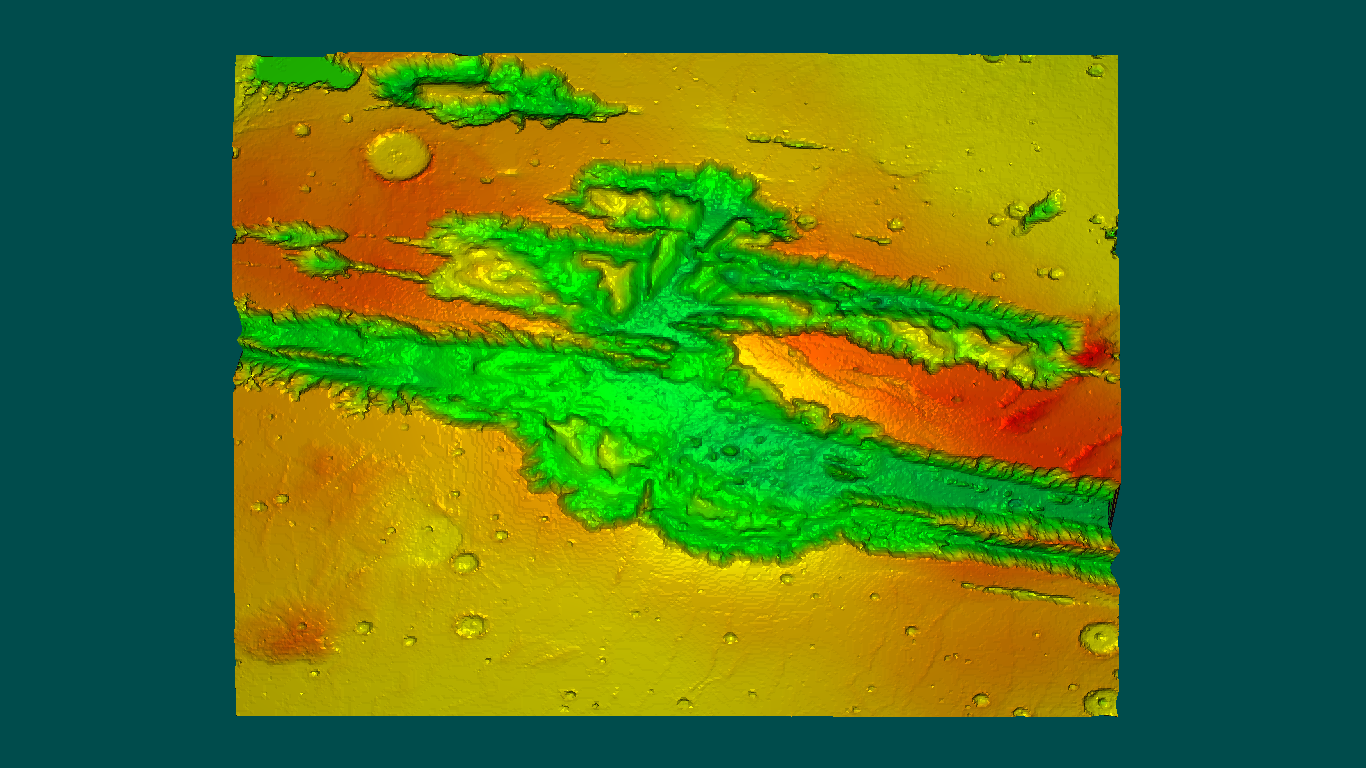
\includegraphics[width=\textwidth]{figures/myterrain.png}
	\caption[Coloreado de Valles Marineris.]{Coloreado de Valles Marineris.
	Modelo:~\cite{NASA}}
	\label{fig:myterrain}
\end{figure}

Para este problema, descrito en la sección~\ref{ref:terrain}, se ha elaborado un
vertex shader y un fragment shader. Partiendo del modelo de un terreno existen
dos posibilidades: que las alturas vengan codificadas en forma de textura o que
venga implícitamente en la posición de los vértices. En este último caso, en la
aplicación se lee el valor más alto y el valor más bajo en el eje $y$ para
realizar la coloración. 

Así, el vertex shader toma como entrada la posición y los normales de los
vértices, sacados de un modelo tridimensional.

\begin{verbatim}
    layout (location = 0) in vec3 aPos;
    layout (location = 1) in vec3 aNormal;
\end{verbatim}

Como solo se están utilizando el vertex shader y fragment shader, la salida del
vertex shader se da como entrada al fragment shader. Esta salida corresponde al
normal, que es el mismo que entra; la posición del fragmento y el color del
fragmento. Estas dos últimas variables se calculan en el vertex shader
utilizando la altura máxima y mínima del modelo, que se pasan mediante variables
\verb|uniform|.  Además, con el fin de mejorar el rendimiento, las
transformaciones de los vértices, que vienen dadas por las matrices de modelo,
vista y proyección, se calculan también en este shader. El siguiente fragmento
de código muestra las salidas del vertex shader junto con las variables
\verb|uniform| utilizadas:

\begin{verbatim}
    out vec3 vNormal;
    out vec3 vFragPos;
    out vec3 vFragColor;
    
    uniform float uMaxHeight;
    uniform float uMinHeight;
    uniform mat4 uModel;
    uniform mat4 uView;
    uniform mat4 uProjection;
\end{verbatim}

El color del fragmento se calcula realizando una interpolación entre el valor
máximo de altura(rojo), el valor tres cuartos de altura(amarillo), el valor
medio de la altura(verde) y el valor mínimo de altura(azul). El código siguiente
muestra el cálculo del color de un fragmento entre la altura máxima y los tres
cuartos:

\begin{verbatim}
    if (aPos.z > threecuarters) {
        alpha = smoothstep(uMaxHeight, threecuarters, aPos.z);	
        vFragColor = mix(RED, YELLOW, alpha);	
    }
\end{verbatim}

Asimismo, para calcular la posición del fragmento se utiliza el siguiente
código:

\begin{verbatim}		
    vFragPos = vec3(uModel * vec4(aPos, 1.0)); 
    gl_Position =  uProjection * uView * vec4(vFragPos, 1.0);
\end{verbatim}

Esto es todo lo que realiza el vertex shader, y sería suficiente para renderizar
el terreno coloreado. Sin embargo, con el fin de darle más realismo, en esta
ocasión se ha utilizado el fragment shader para dotar de iluminación a la
escena. Así, se han utilizado los normales, la posición y el color del fragmento
para elaborar un modelo de iluminación ADS~\cite{Bailey}. Esto es todo lo que
realiza el fragment shader, quedándonos lo siguiente:

\begin{verbatim}
    //Ambient
    vec3 ambient = uLight.ambient * vFragColor; 
    
    //Difuse
    vec3 norm = normalize(uNormalMatrix * vNormal);
    vec3 lightDir = normalize(uLight.position - vFragPos);
    float diff = max(dot(norm, lightDir), 0.0);
    vec3 diffuse = uLight.diffuse * (diff * vFragColor); 
    
    //Specular
    vec3 viewDir = normalize(uViewPos - vFragPos);
    vec3 reflectDir = reflect(-lightDir, norm); 
    float spec = pow(max(dot(viewDir, reflectDir), 0.0), uShininess);
    vec3 specular = uLight.specular * (spec * vFragColor);
    
    vec3 light = ambient + diffuse + specular;
    fFragColor = vec4(light, 1.0);
\end{verbatim}

El resultado final de la utilización de estos shaders se puede ver en la
figura~\ref{fig:myterrain}, para la que se ha utilizado un modelo de la NASA de
Valles Marineris, un sistema de cañones que recorre el ecuador de marte.

\subsection{Curvas de Bézier}
\label{makereference5.5.2}

Para mostrar las curvas de Bézier se han utilizado un vertex shader, un geometry
shader y un fragment shader. Además, se ha utilizado otro par de shaders para
renderizar tanto los ejes como los puntos de control de la curva. 

En este caso, todo el trabajo se realiza en el geometry shader. El vertex shader
simplemente se encarga de realizar la transformación mediante

\begin{verbatim}
    gl_Position = uProjection * uView * uModel * vec4(aPos, 1.0);
\end{verbatim}
mientras que el fragment shaders solo se encarga de darle color a la curva
mediante la instrucción

\begin{verbatim}
    fFragColor = vec4(ORANGE, 1.0);
\end{verbatim}

Así pues, veamos qué acciones realizar en el geometry shader para conseguir,
mediante los 4 vértices de control, renderizar una curva de Bézier en nuestra
aplicación. Este shader es la versión de~\citet{Bailey}. 

Recordemos de la sección~\ref{ref:GeoShader} que para el shader geométrico ha de
especificarse la primitiva de entrada y la de salida. Esto se realiza mediante
las líneas

\begin{verbatim}
    layout( lines_adjacency ) in;
    layout( line_strip, max_vertices=256 ) out;
\end{verbatim}

Utilizamos \verb|lines_adjacency| puesto que como entrada tomaremos los 4 puntos
de control (y esta es la única entrada que toma 4 puntos. Ver
tabla~\ref{tabla3.1}) y como salida \verb|line_strip| pues queremos renderizar
nuestra curva como una serie de segmentos. El nivel de detalle de nuestra curva
vendrá dado por este número de segmentos, que se especifica mediante una
variable \verb|uniform|.

\begin{verbatim}
    float dt = 1. / float(uNum);
    float t = 0.;
    for( int i  = 0; i <=uNum; i++, t+= dt){
        float omt = 1. -t;
        float omt2 = omt * omt;
        float omt3 = omt * omt2;
        float t2 = t * t;
        float t3 = t * t2;
        vec4 xyzw = omt3 * gl_PositionIn[0] +
        3. * t * omt2 * gl_PositionIn[1] +
        3. * t2 * omt * gl_PositionIn[2] +
        t3 * gl_PositionIn[3];
        gl_Position = xyzw;
        EmitVertex( );
    }
\end{verbatim}

El código anterior supone la totalidad del geometry shader. En él, mediante el
uniform \verb|uNum| indicamos la cantidad de puntos que queremos incluir de la
curva, obteniendo mayor detalle cuanto más alto es este número. El vector
\verb|xyzw| se calcula mediante la ecuación~\eqref{eq:3}. El resultado de este
shader puede verse en la Figura~\ref{fig:mybeziercurve}.

\begin{figure}
	\centering
	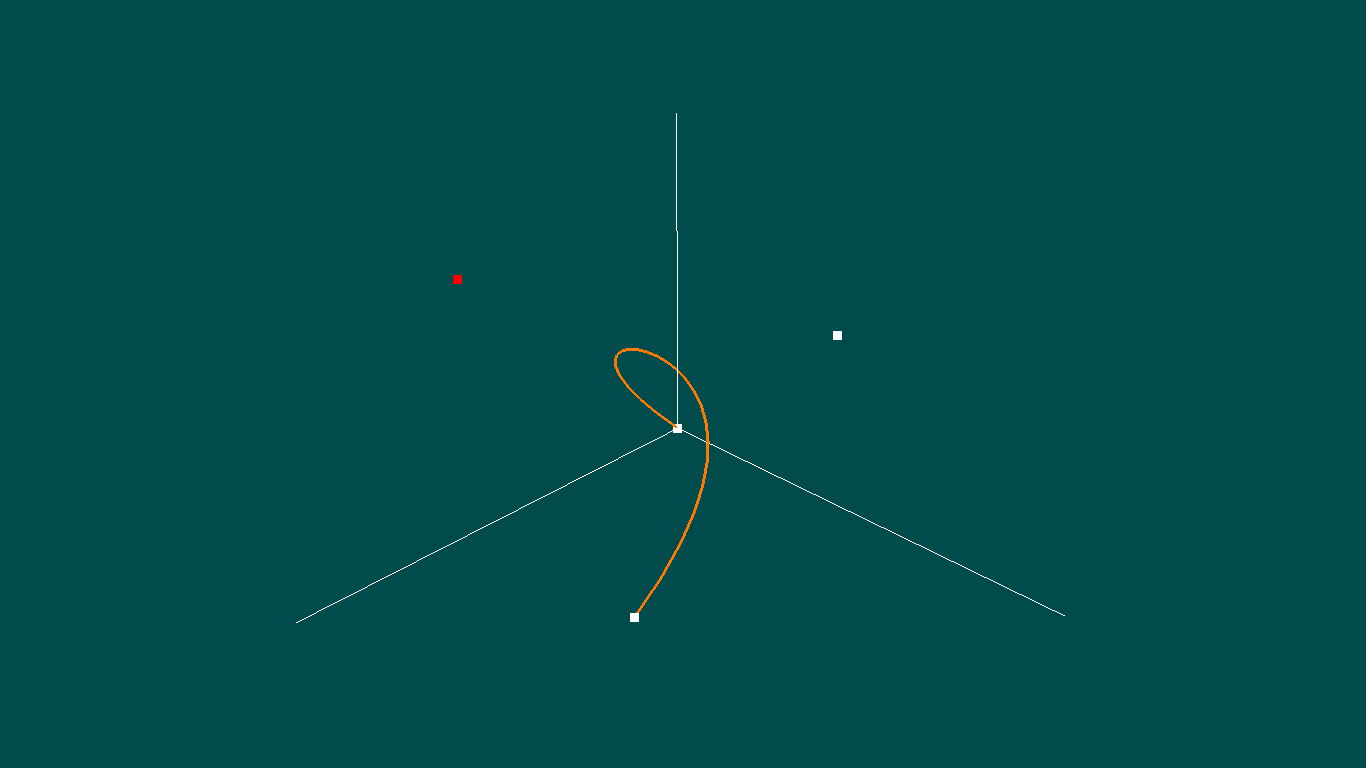
\includegraphics[width=\textwidth]{figures/mybeziercurve.png}
	\caption{Bézier Curve}
	\label{fig:mybeziercurve}
\end{figure}

\subsection{Superficies de Bézier}
\label{makereference5.5.3}

\begin{figure}
	\centering		
	\begin{subfigure}{\textwidth}
		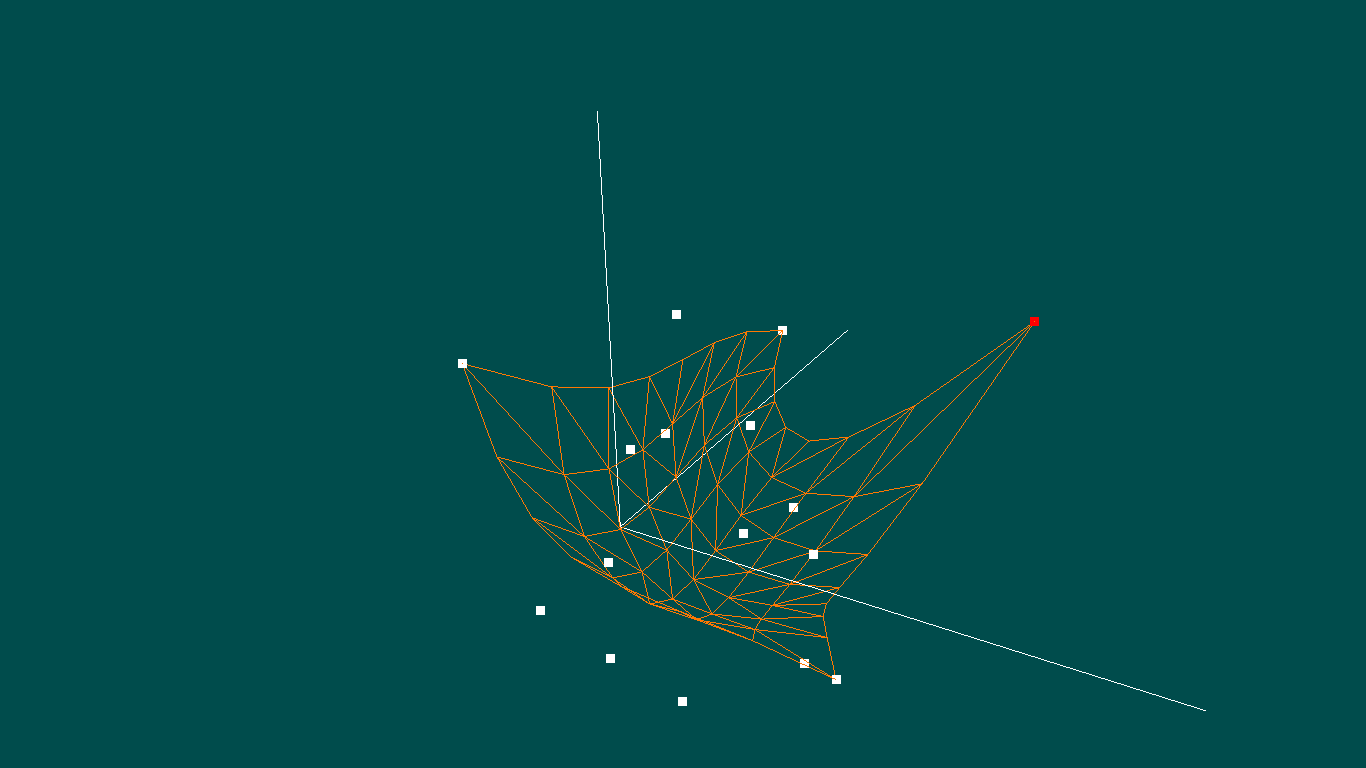
\includegraphics[width=\textwidth]{figures/mybeziersurface1.png}
	\end{subfigure}
	\newline
	\begin{subfigure}{\textwidth}
		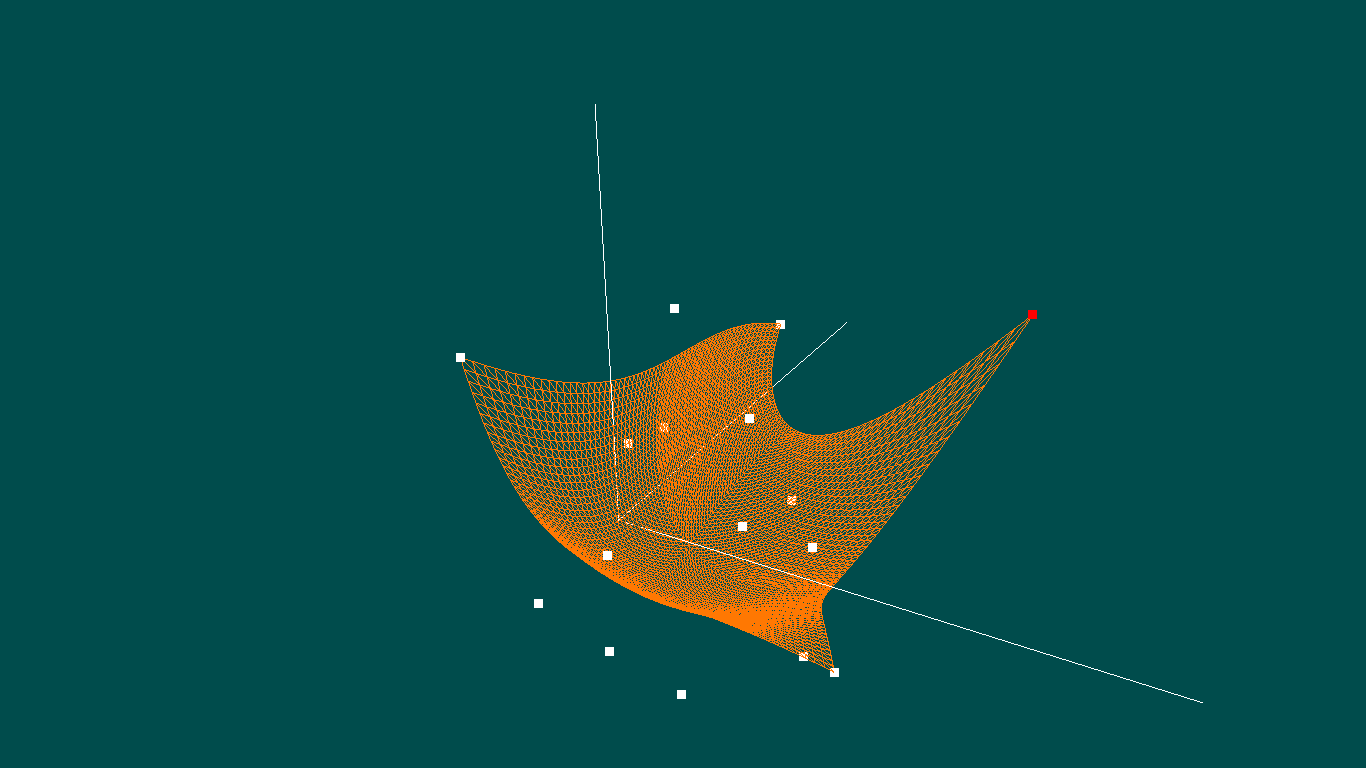
\includegraphics[width=\textwidth]{figures/mybeziersurface2.png}
	\end{subfigure}
	\caption{Superficie de Bézier}
	\label{fig:mybeziersurface}
\end{figure}

En este caso, en lugar de utilizar el shader geométrico como en el caso
anterior, utilizaremos los shaders de teselación. Por tanto, tendremos, al igual
que en el caso anterior, un vertex shader, un tessellation control shader, un
tessellation evaluation shader y un fragment shader, además de los mismos
shaders que en el caso anterior para renderizar los ejes y los puntos de
control. 

El vertex y fragment shader son exactamente iguales que en el caso de la curva
de Bézier, por lo que nos centraremos exclusivamente en los shaders de
teselación. El TCS ha de marcar el nivel de teselación, acorde a lo explicado en
la sección~\ref{ref:TesShaders}, y, debido a que queremos utilizar cuadriláteros
y guiándonos por la Figura~\ref{fig:quadlevels}, debemos especificar los
siguientes niveles de teselación:

\begin{verbatim}
    gl_TessLevelOuter[0] = gl_TessLevelOuter[2] = uOuter02;
    gl_TessLevelOuter[1] = gl_TessLevelOuter[3] = uOuter13;
    gl_TessLevelInner[0] = uInner0;
    gl_TessLevelInner[1] = uInner1;
\end{verbatim}

Además se pasa al TES la posición del vértice dentro del parche mediante la
instrucción:

\begin{verbatim}
    gl_out[ gl_InvocationID ].gl_Position =
        gl_in[ gl_InvocationID ].gl_Position;
\end{verbatim}

En el TES es donde realmente se realizan los cálculos necesarios para obtener la
superficie de Bézier. El siguiente código, que realiza el cálculo de la
ecuación~\eqref{eq:6} es una versión simplificada del que se puede encontrar
en~\citet{Bailey}. Este último utiliza también las propiedades de las derivadas
de las superficies de Bézier para calcular el normal con el fin de utilizar un
modelo de luz como el utilizado en~\ref{makereference5.5.1}.

\begin{verbatim}
    vec4 p00 = gl_in[0].gl_Position;
    vec4 p10 = gl_in[1].gl_Position;
    vec4 p20 = gl_in[2].gl_Position;
    vec4 p30 = gl_in[3].gl_Position;
    vec4 p01 = gl_in[4].gl_Position;
    vec4 p11 = gl_in[5].gl_Position;
    vec4 p21 = gl_in[6].gl_Position;
    vec4 p31 = gl_in[7].gl_Position;
    vec4 p02 = gl_in[8].gl_Position;
    vec4 p12 = gl_in[9].gl_Position;
    vec4 p22 = gl_in[10].gl_Position;
    vec4 p32 = gl_in[11].gl_Position;
    vec4 p03 = gl_in[12].gl_Position;
    vec4 p13 = gl_in[13].gl_Position;
    vec4 p23 = gl_in[14].gl_Position;
    vec4 p33 = gl_in[15].gl_Position;
    
    float u = gl_TessCoord.x;
    float v = gl_TessCoord.y;
    
    float bu0 = (1.-u) * (1.-u) * (1.-u);
    float bu1 = 3. * u * (1.-u) * (1.-u);
    float bu2 = 3. * u * u * (1.-u);
    float bu3 = u * u  * u;
    
    float bv0 = (1.-v) * (1.-v) * (1.-v);
    float bv1 = 3. * v * (1.-v) * (1.-v);
    float bv2 = 3. * v * v * (1.-v);
    float bv3 = v * v * v;
    
    gl_Position = 
          bu0 * ( bv0*p00 + bv1*p01 + bv2*p02 + bv3*p03 )
        + bu1 * ( bv0*p10 + bv1*p11 + bv2*p12 + bv3*p13 )
        + bu2 * ( bv0*p20 + bv1*p21 + bv2*p22 + bv3*p23 )
        + bu3 * ( bv0*p30 + bv1*p31 + bv2*p32 + bv3*p33 );

\end{verbatim}

El resultado de estos shaders se puede ver en la
Figura~\ref{fig:mybeziersurface}.

\subsection{Sólidos de revolución}
\label{makereference5.5.4}

En este caso, de nuevo, tanto el vertex shader como el fragment shader son los
más simples posible, como en los casos anteriores. Todo el trabajo recae en el
geometry shader. Así, dados los vértices que forman una curva, se van generando
vértices en torno al eje $y$, tantos como indica la variable \verb|uNum|. El
resultado de revolucionar una curva en torno al eje $y$ puede verse en la
Figura~\ref{fig:myrevolution}. El código del geometry shader utilizado es el
siguiente:

\begin{verbatim}
    for( int i  = 0; i <= uNum; i++){
        float grados = 2.0*PI / uNum * i;
        
        gl_Position = gl_in[0].gl_Position;
        gl_Position.x = cos(grados)*gl_PositionIn[0].x 
		                + sin(grados)*gl_PositionIn[0].z;
        gl_Position.z = cos(grados)*gl_PositionIn[0].z 
		                - sin(grados)*gl_PositionIn[0].x;

        gl_Position = uProjection * uView * uModel * gl_Position;
        EmitVertex( );
        
        gl_Position = gl_PositionIn[1];
        gl_Position.x = cos(grados)*gl_PositionIn[1].x 
		                + sin(grados)*gl_PositionIn[1].z;
        gl_Position.z = cos(grados)*gl_PositionIn[1].z 
		                - sin(grados)*gl_PositionIn[1].x;

        gl_Position = uProjection * uView * uModel * gl_Position;
        EmitVertex( );
    }
\end{verbatim}

\begin{figure}[ht]
	\centering		
	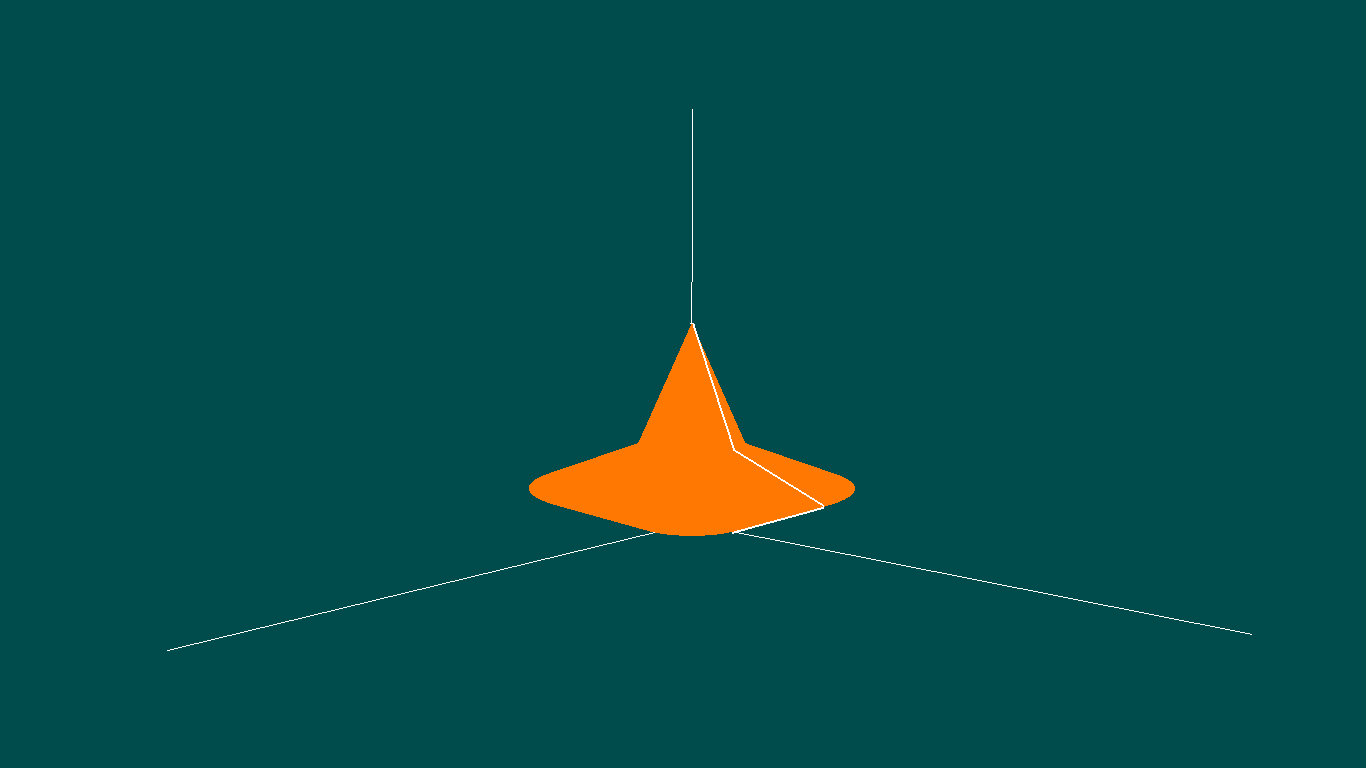
\includegraphics[width=\textwidth]{figures/myrevolution.png}
	\caption{Sólido de revolución}
	\label{fig:myrevolution}
\end{figure}

\subsection{Nube de puntos}
\label{makereference5.5.5}

\begin{figure}[ht]
	\centering	
	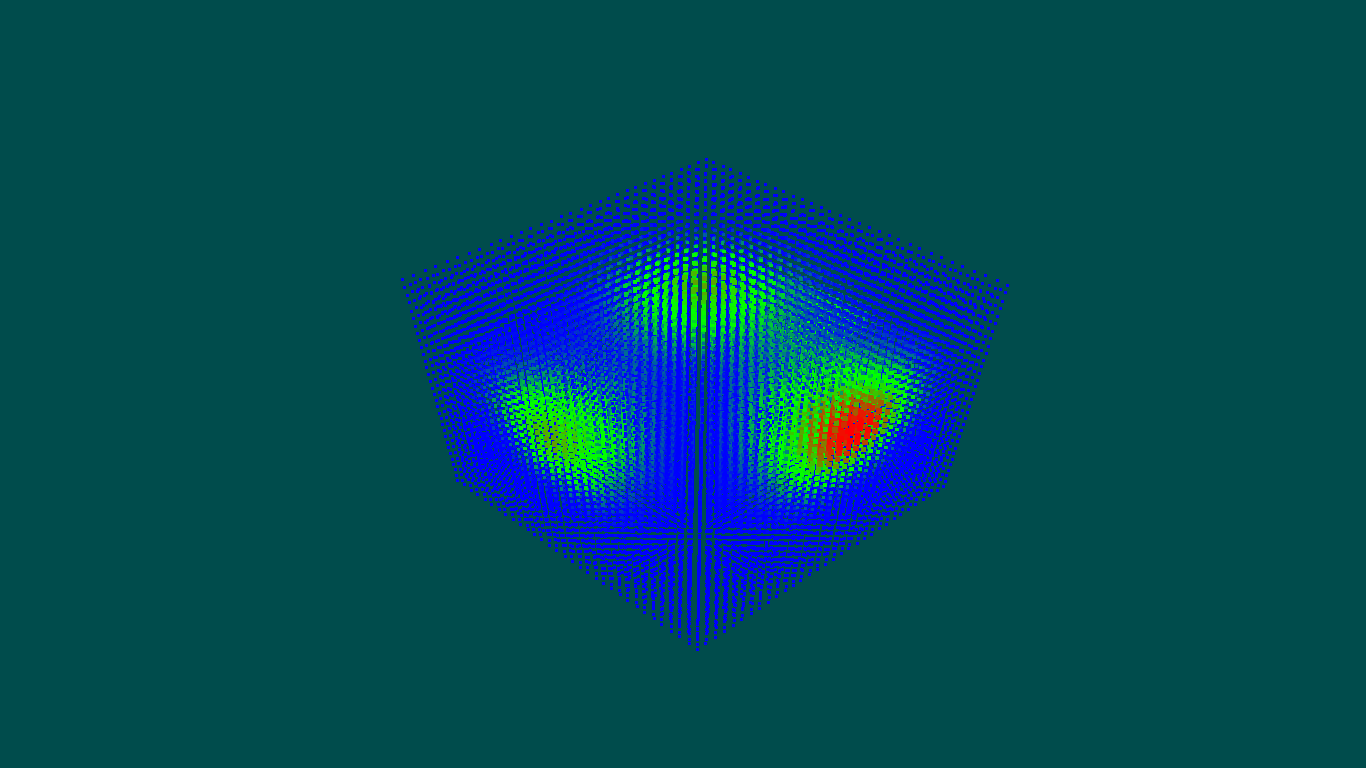
\includegraphics[width=\textwidth]{figures/mycloud.png}
	\caption{Nube de puntos}
	\label{fig:mycloud}
\end{figure}

Para realizar esta visualización se han utilizado únicamente un vertex shader y
un fragment shader. Como entradas, el vertex shader utiliza tanto la posición
del vértice en la nube de puntos como el escalar que representa la información
que queremos visualizar. 

En el vertex shader, además de definir la posición mediante las transformaciones
necesarias, utilizamos la siguiente instrucción

\begin{verbatim}
    gl_PointSize = 2 + pow((smoothstep(0.0, uMaxData, aScalar) + 1), 2);
\end{verbatim}
para definir el tamaño del punto acorde al escalar. Así, los puntos que se
correspondan con escalares más altos tendrán un tamaño mayor. El valor escalar
\verb|aScalar| es pasado también al fragment shader para realizar una coloración
del punto acorde a este valor. 

Además, en el fragment shader se ha declarado la variable \verb|uniform uMax|
que se utiliza para descartar los puntos que tengan valores escalares menores
que él. Así, podemos visualizar de una manera  más efectiva datos por encima de
cierto límite. Este comportamiento puede verse en la Figura~\ref{fig:mycloud2}.
El código para este shader se incluye a continuación.

\begin{verbatim}
    if(vScalar < uMax) discard;	
    float alpha;
    float middle = uMaxData / 2;
    if(vScalar >= middle){
        alpha = smoothstep(middle, uMaxData, vScalar);
        fFragColor = vec4(mix(GREEN, RED, alpha), 1.0f);
    }
    else{
        alpha = smoothstep(0.0, middle, vScalar);
        fFragColor = vec4(mix(BLUE, GREEN, alpha), 1.0f);
    }
\end{verbatim}

\begin{figure}[ht]
	\centering	
	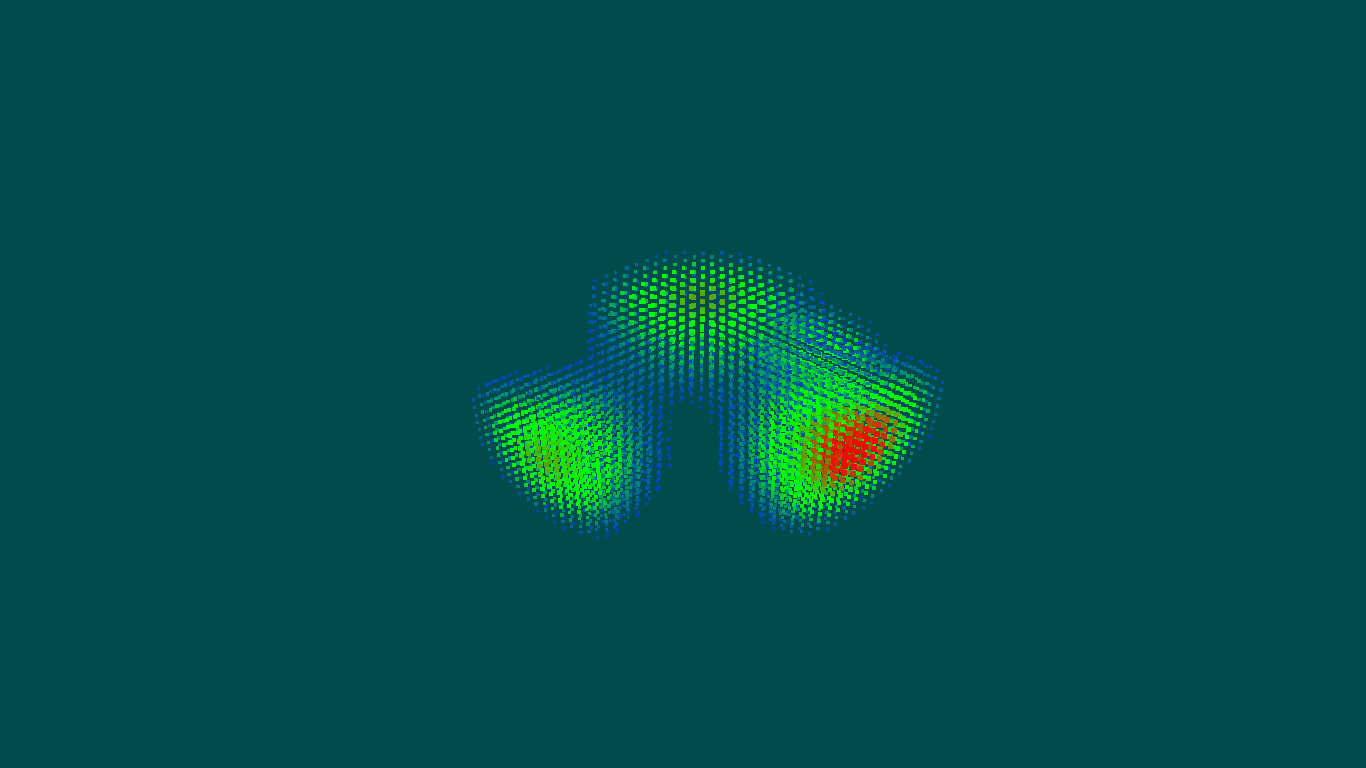
\includegraphics[width=\textwidth]{figures/mycloud2.png}
	\caption{Nube de puntos con valores descartados}
	\label{fig:mycloud2}
\end{figure}

\subsection{Negativo de una imagen}
\label{makereference5.5.6}

\begin{figure}[ht]
	\centering	
	\begin{subfigure}{0.45\textwidth}
		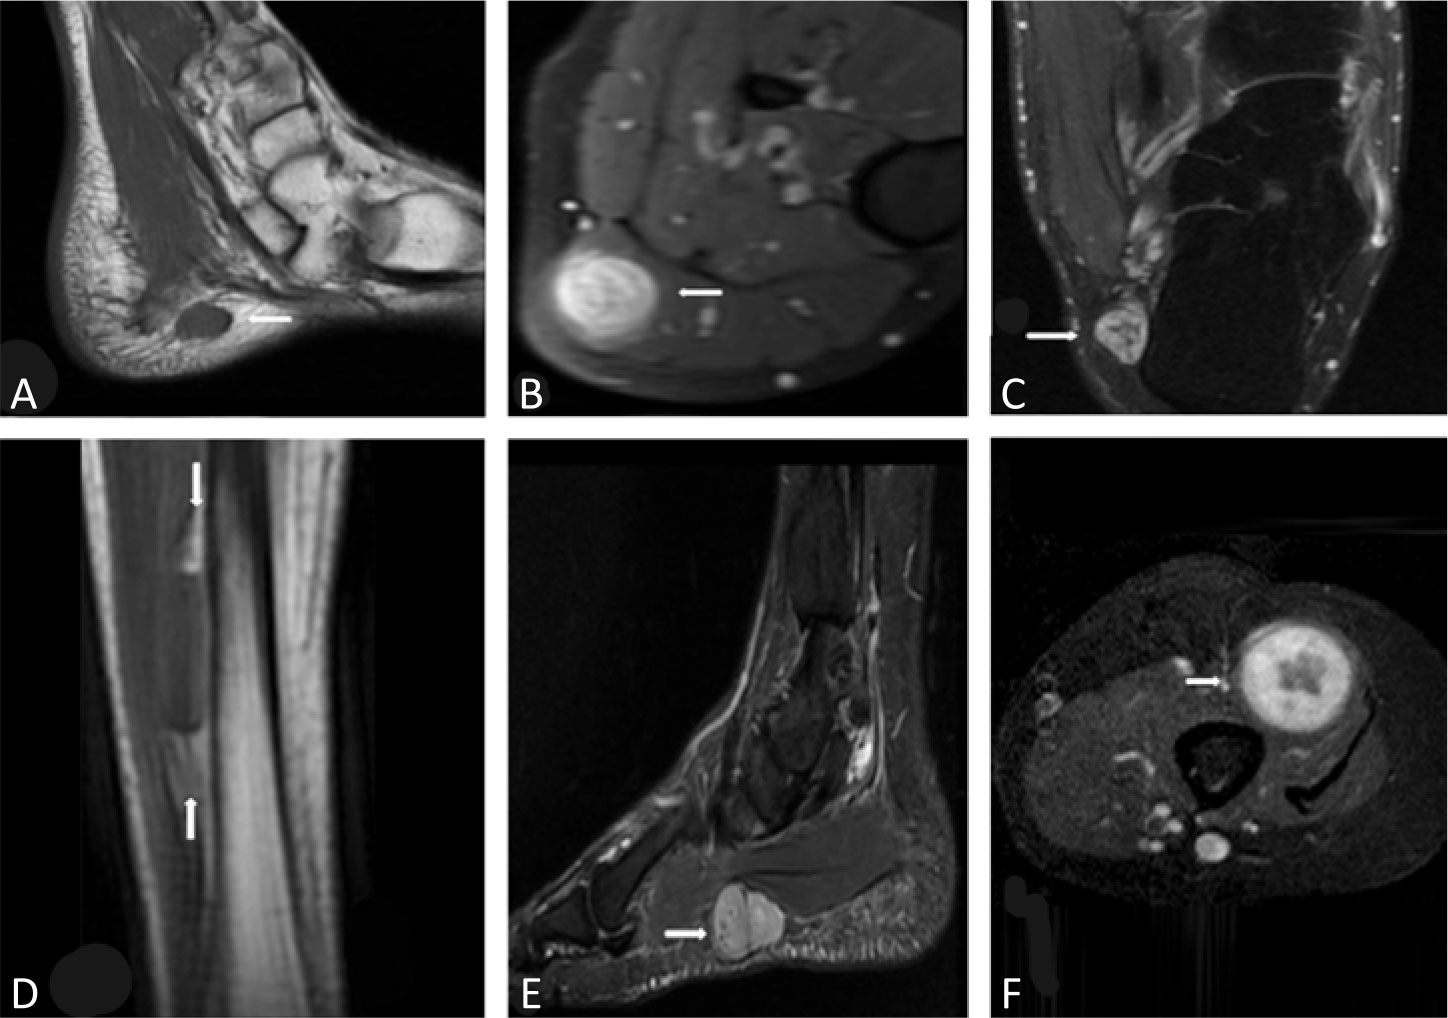
\includegraphics[height=8cm,width=\textwidth]{figures/mynegative00.jpg}
		\caption{Imagen original}
	\end{subfigure}
	\hfill
	\begin{subfigure}{0.45\textwidth}
		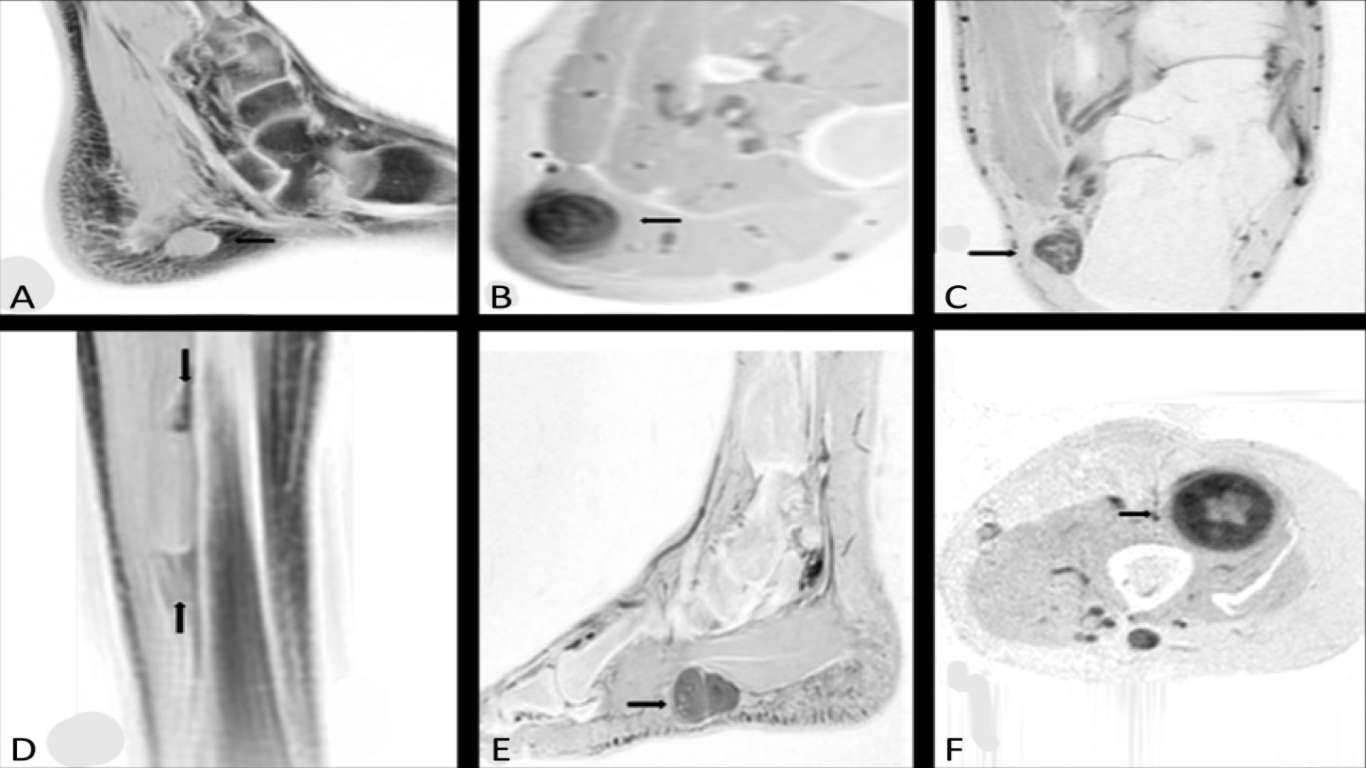
\includegraphics[height=8cm,width=\textwidth]{figures/mynegative01.png}
		\caption{Negativo}
	\end{subfigure}
	\caption[Negativo de una imagen.]{Negativo de una imagen.
	Fuente:~\cite{negativeimage}}
	\label{fig:mynegative}
\end{figure}

En este caso, al tratarse de una imagen, los únicos elementos que necesitamos
son cuatro vértices cuya posición se corresponda con cada una de las esquinas de
la imagen y la textura para la imagen. Así pues, el vertex shader toma como
entrada la posición de estos cuatro vértices junto a las coordenadas que le
corresponden en la textura. Estas coordenadas de textura se definen en el
intervalo $(0,1)\times(0,1)$, siendo el punto $(0,0)$ la esquina inferior
izquierda de la textura y el punto $(1,1)$ la esquina superior derecha. Con
estos datos, el vertex shader escribe la posición de los cuatro vértices y pasa
las coordenadas de textura al fragment shader, que es el que las utilizará. 

El fragment shader, por su parte, obtiene el color original de los fragmentos
con la instrucción

\begin{verbatim}
    vec3 irgb = texture( texture1, vTexCoords ).rgb;
\end{verbatim}
para posteriormente computar el color negativo y escribirlo como salida para el
pixel. Esta tarea se realiza con las siguientes instrucciones:

\begin{verbatim}
    vec3 neg = vec3(1.,1.,1.) - irgb;
    fFragColor = vec4( mix( irgb, neg, uT ), 1. );
\end{verbatim}

Una muestra del funcionamiento de este shader se puede encontrar en la
Figura~\ref{fig:mynegative}.

\subsection{Line Integral Convolution}
\label{makereference5.5.8}

El caso del Line Integral Convolution presenta un problema a la hora de realizar
mediante un shader los cálculos necesarios. Esto se debe a que, como hemos visto
anteriormente, necesitamos, para calcular la línea de flujo, los valores del
campo vectorial de los demás vértices, algo que no podemos, a priori, obtener en
un shader. La solución para este problema consiste en codificar en forma de
textura la información del campo vectorial asociado al problema. 

\begin{figure}[b]
	\centering	
	\begin{subfigure}{0.7\textwidth}
			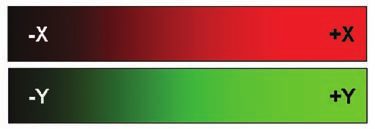
\includegraphics[width=\textwidth]{figures/lictexture2.png}	
	\end{subfigure}
	\begin{subfigure}{0.28\textwidth}
			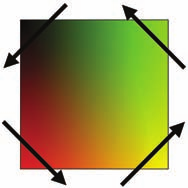
\includegraphics[width=\textwidth]{figures/lictexture.png}	
	\end{subfigure}
	\caption[LIC - Información del campo vectorial codificado en una
	textura.]{LIC - Información del campo vectorial codificado en una textura.
	Fuente:~\cite{Bailey}}
	\label{fig:lictexture}
\end{figure}

Para ello, como se explica en~\citet{Bailey} y como se puede observar en la
Figura~\ref{fig:lictexture}, se asocia a cada punto del campo un color
dependiendo de los valores de las componentes vectoriales de dicho punto. A
mayor valor de la coordenada $x$ se le asocia un valor más alto del color rojo
siguiendo el convenio RGB. Similarmente, a mayor valor de la coordenada $y$ se
le asocia un valor mayor del color verde. 

\begin{figure}
	\centering	
	\begin{subfigure}{0.45\textwidth}
		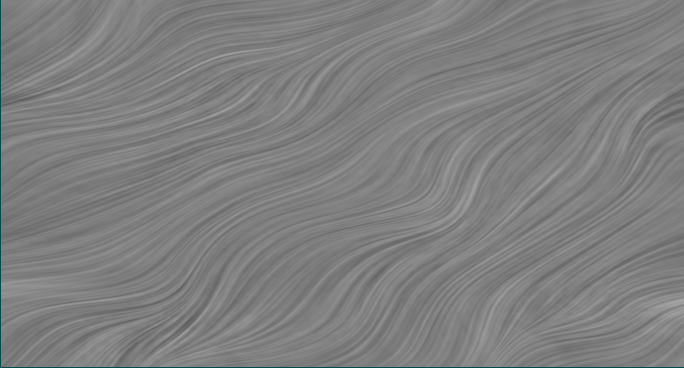
\includegraphics[height=\textwidth,width=\textwidth]{figures/mylic.png}
		\caption{Lic para el flujo vectorial de debajo.}
		\label{fig:mylic1}
	\end{subfigure}
	\hfill
	\begin{subfigure}{0.45\textwidth}
		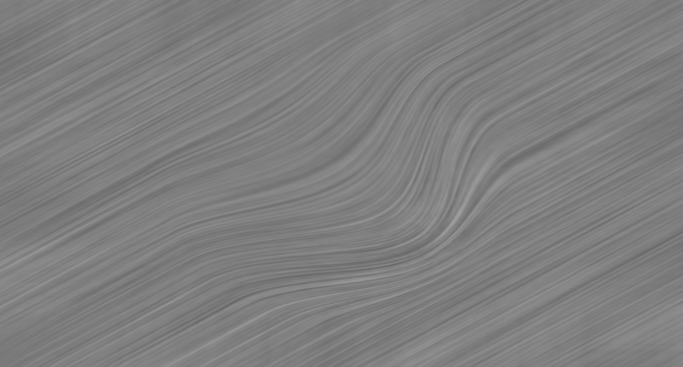
\includegraphics[height=\textwidth,width=\textwidth]{figures/mylic2.png}
		\caption{Lic para el flujo vectorial de debajo.}
		\label{fig:mylic2}
	\end{subfigure}
	\newline 
	\par\bigskip\par\bigskip
	\begin{subfigure}{0.45\textwidth}
		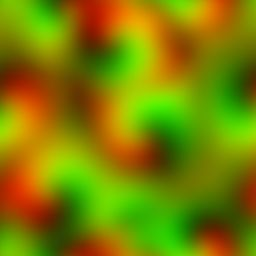
\includegraphics[height=\textwidth,width=\textwidth]{figures/mylic3.jpg}
		\caption{Flujo vectorial codificado en textura.}
		\label{fig:mylic3}
	\end{subfigure}
	\hfill
	\begin{subfigure}{0.45\textwidth}
		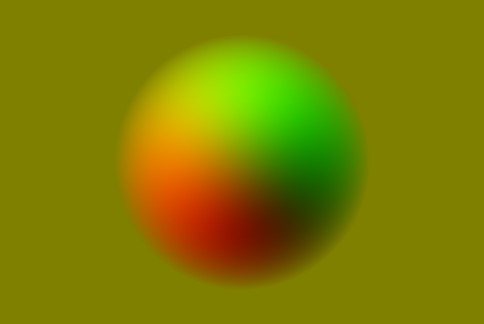
\includegraphics[height=\textwidth,width=\textwidth]{figures/mylic4.png}
		\caption{Flujo vectorial codificado en textura.}
		\label{fig:mylic4}
	\end{subfigure}
	\caption{Line Integral Convolution.}
	\label{fig:mylic}
\end{figure}

Las texturas con estos valores así calculados tienen un aspecto similar al de las
Figuras~\ref{fig:mylic3} y~\ref{fig:mylic4}, dependiendo del flujo vectorial
subyacente.

Para esta técnica necesitaremos solo un vertex shader y un fragment shader. El
vertex shader toma de nuevo la posición de los vértices, que en este caso se
trata de una malla de $256\times 256$ vértices y las coordenadas de textura de
cada uno de ellos. Este shader simplemente pasa las coordenadas de textura al
fragment shader y escribe la posición del vértice. 

El fragment shader toma las coordenadas de textura procedentes del vertex shader
y realiza las operaciones explicadas en la sección~\ref{ref:lic}. Primero
realiza, para cada vértice, el cómputo de la línea de flujo mediante el método
de Runge-Kutta de orden 4. Para este método se define el tamaño del paso
mediante la variable \verb|stp| y la longitud de la línea de flujo que queremos
calcular mediante la variable \verb|uniform uLength|.

\begin{verbatim}
    vec3 color = texture( texture1, vTexCoords ).rgb;
    vec2 st = vTexCoords;
    float stp = 0.00281;

    // Cálculo de la línea de flujo en dirección positiva
    for( int i = 0; i < uLength; i++ )
    {
        vec2 k1 = texture( texture2, st ).xy;
        vec2 k2 = texture( texture2, st + k1*stp/2 ).xy;
        vec2 k3 = texture( texture2, st + k2*stp/2 ).xy;
        vec2 k4 = texture( texture2, st + k3*stp).xy;
        vec2 ks = k1 + 2*k2 + 2*k3 + k4;
        st += stp/6*ks;
        st = clamp( st, 0., 1. );
        color += vec3( texture( texture1, st ) );
    }

    // Cálculo de la línea de flujo en dirección negativa
    st = vTexCoords;
    for( int i = 0; i < uLength; i++ )
    {
        vec2 k1 = texture( texture2, st ).xy;
        vec2 k2 = texture( texture2, st - k1 * stp / 2 ).xy;
        vec2 k3 = texture( texture2, st - k2 * stp / 2 ).xy;
        vec2 k4 = texture( texture2, st - stp*k3).xy;
        vec2 ks = k1 + 2*k2 + 2*k3 + k4;
        st -= stp/6*ks;
        st = clamp( st, 0., 1. );
        color += vec3( texture( texture1, st ) );
    }
    color /= float(2*uLength + 1); 
\end{verbatim}

En este shader se ha omitido el cálculo de los pesos, tomando como valor para
ellos $1$ en todos los casos y dividiendo por el número de puntos en la línea
de flujo. Con todo esto en cuenta, el resultado final se puede observar en la
Figura~\ref{fig:mylic}.

\subsection{Uso de la aplicación}
\label{subsection:uso}

Una vez visto el diseño de la aplicación y los shaders utilizados, se presenta
el modo de utilización de la aplicación. Una vez conseguido el ejecutable, para
esta explicación llamado \verb|tfg| se debe ejecutar con alguno de los modos de
visualización explicados anteriormente. Cada uno de estos modos permite unas
opciones de visualización diferentes, que se explican a continuación.

Además, todos los modos comparten el movimiento de la cámara, que es el
siguiente:

\begin{itemize}
		\item \verb|Esc| - Salir.
		\item \verb|w| - Mover la cámara hacia delante.
		\item \verb|s| - Mover la cámara hacia atrás.
		\item \verb|d| - Mover la cámara hacia la derecha.
		\item \verb|a| - Mover la cámara hacia la izquierda.
\end{itemize}

Junto con el movimiento del ratón, que cambia el objetivo al que apunta la
cámara, y la ruleta del ratón, que permite hacer y deshacer zoom.

\subsubsection{Visualización de Terrenos}

\verb|$ ./tfg terrain|

Opciones: No tiene opciones especiales.

\subsubsection{Curva de Bézier}

\verb|$ ./tfg bezier|

La aplicación permite aumentar y disminuir el número de vértices de la curva,
así como mover los puntos de control.
Opciones:

\begin{itemize}
		\item \verb|\textvisiblespace| - Seleccionar siguiente vértice.
		\item \verb|\uparrow| - Aumentar número de segmentos.
		\item \verb|\downarrow| - Disminuir número de segmentos.
		\item \verb|m| - Cambiar modo cámara/selección.
		\item \verb|Ratón izquierdo| - Seleccionar vértice. (Solo modo
				selección).
		\item \verb|Ratón derecho| - Mover vértice seleccionado. (Solo modo
				selección).
		\item \verb|x| - Mover el vértice seleccionado en la dirección $+x$.
		\item \verb|y| - Mover el vértice seleccionado en la dirección $+y$.
		\item \verb|z| - Mover el vértice seleccionado en la dirección $+z$.
		\item \verb|Shift + x| - Mover el vértice seleccionado en la dirección $-x$.
		\item \verb|Shift + y| - Mover el vértice seleccionado en la dirección $-y$.
		\item \verb|Shift + z| - Mover el vértice seleccionado en la dirección $-z$.
\end{itemize}

\subsubsection{Superficie de Bézier}

\verb|$ ./tfg bsurface|

La aplicación permite aumentar y disminuir el grado de teselación de la
superficie, así como mover los puntos de control.  
Opciones:

\begin{itemize}
		\item \verb|\textvisiblespace| - Seleccionar siguiente vértice.
		\item \verb|\uparrow| - Aumentar grado de teselación.
		\item \verb|\downarrow| - Disminuir grado de teselación.
		\item \verb|t| - Activar el modo wireframe
		\item \verb|u| - Desactivar el modo wireframe
		\item \verb|m| - Cambiar modo cámara/selección.
		\item \verb|Ratón izquierdo| - Seleccionar vértice. (Solo modo
				selección).
		\item \verb|Ratón derecho| - Mover vértice seleccionado. (Solo modo
				selección).
		\item \verb|x| - Mover el vértice seleccionado en la dirección $+x$.
		\item \verb|y| - Mover el vértice seleccionado en la dirección $+y$.
		\item \verb|z| - Mover el vértice seleccionado en la dirección $+z$.
		\item \verb|Shift + x| - Mover el vértice seleccionado en la dirección $-x$.
		\item \verb|Shift + y| - Mover el vértice seleccionado en la dirección $-y$.
		\item \verb|Shift + z| - Mover el vértice seleccionado en la dirección $-z$.
\end{itemize}

\subsubsection{Nube de puntos}

\verb|$ ./tfg cloud|

Opciones:

\begin{itemize}
		\item \verb|\uparrow| - Aumentar límite para el escalar.
		\item \verb|\downarrow| - Disminuir límite para el escalar.
\end{itemize}

\subsubsection{Negativo}

\verb|$ ./tfg negative|

Opciones: No tiene opciones especiales

\subsubsection{Sólido de revolución}

\verb|$ ./tfg revolution|

Opciones:

\begin{itemize}
		\item \verb|\uparrow| - Aumentar número de vértices de revolución.
		\item \verb|\downarrow| - Disminuir número de vértices de revolución.
		\item \verb|t| - Activar el modo wireframe
		\item \verb|u| - Desactivar el modo wireframe
\end{itemize}

\subsubsection{Line Integral Convolution}

\verb|$ ./tfg lic|

Opciones:

\begin{itemize}
		\item \verb|\uparrow| - Aumentar longitud de la línea de flujo.
		\item \verb|\downarrow| - Disminuir longitud de la línea de flujo.
\end{itemize}
